\documentclass[11pt, openany]{article}
\usepackage[utf8]{inputenc}
\usepackage[T1]{fontenc}

\usepackage{natbib}
\usepackage{graphicx}
\usepackage{xcolor}


\setlength{\parindent}{0cm}
\setlength{\parskip}{1ex plus 0.5ex minus 0.2ex}
\newcommand{\hsp}{\hspace{20pt}}
\newcommand{\HRule}{\rule{\linewidth}{0.5mm}}

\usepackage[a4paper]{geometry}
\geometry{hscale=0.85,vscale=0.85,centering}
\usepackage{listings}

\lstdefinelanguage
   [x64]{Assembler}     % add a "x64" dialect of Assembler
   [x86masm]{Assembler} % based on the "x86masm" dialect
   % with these extra keywords:
   {morekeywords={CDQE,CQO,CMPSQ,CMPXCHG16B,JRCXZ,LODSQ,MOVSXD, %
                  POPFQ,PUSHFQ,SCASQ,STOSQ,IRETQ,RDTSCP,SWAPGS, %
                  rax,rdx,rcx,rbx,rsi,rdi,rsp,rbp, %
                  r8,r8d,r8w,r8b,r9,r9d,r9w,r9b, %
                  r10,r10d,r10w,r10b,r11,r11d,r11w,r11b, %
                  r12,r12d,r12w,r12b,r13,r13d,r13w,r13b, %
                  r14,r14d,r14w,r14b,r15,r15d,r15w,r15b}} % etc.
\lstset{language=[x64]Assembler}


\begin{document}

\begin{titlepage}
\begin{sffamily}
\begin{center}

% Upper part of the page. The '~' is needed because \\
% only works if a paragraph has started.

\includegraphics[scale=0.4]{images/LOGO_SU_HORIZ_SEUL_RVB.png}~\\[1.5cm]

\textsc{\textmd{\LARGE sorbonne université UPMC}}\\[2cm]

\textsc{\textmd{\Large Rapport CompilationAvanée}}\\[1.5cm]

% Title
\HRule \\[0.4cm]
\textbf{\Large  OPTIMISATION D'UN CODE
ASSEMBLEUR COMPILATION AVANCEE \\[0.4cm] }

\HRule \\[1cm]

% Author and supervisor
\begin{minipage}{0.4\textwidth}
\begin{flushleft} \normalsize
Katia AMICHI(3603567)\\
Nadir BELAROUCI(3704056)\\
\end{flushleft}
\end{minipage}

\vfill

% Bottom of the page
{Lundi 13 mai 2019}

\end{center}
\end{sffamily}
\end{titlepage}

\newpage

\tableofcontents

\newpage

\section{Introduction}
Pour ce projet, nous implémentons un ensemble de fonctions permettant de traiter et d'optimiser du code assembleur. Ainsi, nous structurerons le
code en délimitant les blocs de base puis nous analyserons les
dépendances entre les instructions et puis nous effectuerons le renommage des registres. Enfin nous proposerons des optimisations qui ont pour but de limiter les dépendances et d'améliorer l’ordonnancement des instructions.

Ce projet est implémenté en C++.

\section{Fonctionnalités implémentées}

Nous avons implémenté, testé et vérifié manuellement toutes les fonctions suivantes:

\begin{enumerate}
    \item Le calcul des blocs de base.
    \item Le calcul des successeurs et prédecesseurs des blocs de bases.
    \item Le calcul du CFG.
    \item Le calcul des blocs dominants.
    \item Le calcul des dépendances.
    \item Le calcul du nombre de cycles.
    \item Le calcul des registres USE et DEF, LiveIn et LiveOut.
    \item Le calcul des registres DefLiveOut.
    \item Le renommage de registres.
\end{enumerate}

\section{Analyses expérimentales}
\subsection{Analyse complète des fonctions implementées}
\textbf{Fichier de test: test\_td.s (code assembleur vue en td2 voir annexe \ref{chap:TestTd2}) }

\newpage
\subsubsection{test\_decoupage\_bb (comput\_basic\_bloc)}

Où on retrouve bien le découpage souhaité.

\begin{lstlisting}
nombre de fonctions : 1
FONCTION 0
Affichage des blocs de base 
Begin BB0
main:
    i0 lw $4,0($6)
    i1 lw $2,0($4)
    i2 add $5,$14,$2
    i3 ori $10,$6,0
    i4 sw $5,0($10)
    i5 lw $2,65524($10)
    i6 addi $5,$2,4
    i7 bne $5,$2,$l5
    i8 add $0,$0,$0
End BB0

Begin BB1
$l4:
    i0 lw $4,0($6)
    i1 lw $2,0($7)
    i2 add $5,$4,$2
    i3 sw $5,0($6)
    i4 addiu $12,$8,2
    i5 addiu $7,$12,1
    i6 bne $7,$0,$l5
    i7 add $0,$0,$0
End BB1

Begin BB2
    i0 sub $6,$0,$5
    i1 sll $6,$3,4
    i2 addiu $5,$6,65534
    i3 sw $15,12($7)
    i4 sw $10,65532($6)
    i5 j $l4
    i6 add $0,$0,$0
End BB2

Begin BB3
$l5:
    i0 sub $8,$10,$15
    i1 sll $10,$10,4
    i2 sw $8,8($7)
    i3 add $10,$8,$10
    i4 sw $10,12($7)
    i5 jr $31
    i6 add $0,$0,$0
End BB3
\end{lstlisting}

\subsubsection{test\_liens\_bb (compute\_succ\_pred\_BB)}
\begin{lstlisting}
test du BB 0
nb de predecesseurs : 0
nb de successeurs : 2
 succ 0 : BB1
 succ 1 : BB3

test du BB 1
nb de predecesseurs : 2
 pred 0 : BB0
 pred 1 : BB2
nb de successeurs : 2
 succ 0 : BB2
 succ 1 : BB3

test du BB 2
nb de predecesseurs : 1
 pred 0 : BB1
nb de successeurs : 1
 succ 0 : BB1

test du BB 3
nb de predecesseurs : 2
 pred 0 : BB0
 pred 1 : BB1
nb de successeurs : 0

\end{lstlisting}


on a vérifié cette fonction grâce au plot généré à partir des fichiers solutions fournis, que nous retrouvons en Annexe \ref{chap:cfg} .\\
Les résultats obtenus:
\begin{lstlisting}

nombre de fonctions : 1
Dominants pour BB0 :  BB0
Dominants pour BB1 :  BB0 BB1
Dominants pour BB2 :  BB0 BB1 BB2
Dominants pour BB3 :  BB0 BB3
\end{lstlisting}

\subsubsection{test\_loops.cpp (compute\_loops)}
Pour ce code on a trouvé une boucle entre BB1 et BB2 qu'on peut voir dans le cfg dans l'annexe \ref{chap:cfg}
.

\subsubsection{ test\_dependances\_instr (comput\_pred\_succ)}
\begin{lstlisting}
---------- BB 0 -----------
Affichage dependance des instructions du BB 0
i0 -> i4 : MEMDEP
i0 -> i1 : RAW
i1 -> i4 : MEMDEP
i1 -> i2 : RAW
i2 -> i5 : WAR
i2 -> i4 : RAW
i3 -> i5 : RAW
i3 -> i4 : RAW
i4 -> i6 : WAR
i5 -> i7 : RAW
i5 -> i6 : RAW
i6 -> i7 : RAW

---------- BB 1 -----------
Affichage dependance des instructions du BB 1
i0 -> i3 : MEMDEP
i0 -> i2 : RAW
i1 -> i5 : WAR
i1 -> i3 : MEMDEP
i1 -> i2 : RAW
i2 -> i3 : RAW
i3 -> i6 : CONTROL
i4 -> i5 : RAW
i5 -> i6 : RAW

---------- BB 2 -----------
Affichage dependance des instructions du BB 2
i0 -> i2 : WAR
i0 -> i1 : WAW
i1 -> i4 : RAW
i1 -> i2 : RAW
i2 -> i5 : CONTROL
i3 -> i4 : MEMDEP
i4 -> i5 : CONTROL

---------- BB 3 -----------
Affichage dependance des instructions du BB 3
i0 -> i3 : RAW
i0 -> i2 : RAW
i0 -> i1 : WAR
i1 -> i3 : RAW
i1 -> i3 : WAR
i2 -> i5 : CONTROL
i3 -> i4 : RAW
i4 -> i5 : CONTROL
\end{lstlisting}

En vérifiant avec le fichier généré à partir des solutions fournis, on retrouve le même résulat que notre programme. (Annexe A.3)

\subsubsection{test\_nbcycles (nb\_cycles)}

\begin{tabular}{ |p{2.5cm}|p{2.5cm}|p{2.5cm}|p{2.5cm}|  }
 \hline
 BB0 & BB1 & BB2 & BB3\\
 \hline
 13 & 10 & 7 & 7 \\
 \hline
\end{tabular}


\subsubsection{test\_def\_use\_bb (compute\_use\_def) et test\_live\_var (compute\_live\_var)}

\begin{tabular}{ |p{2cm}||p{3cm}|p{3cm}|p{3cm}|p{3cm}|  }
 \hline
   & USE & DEF & LIVEin & LIVEout\\
 \hline
 BBO & \$0 \$6 \$14 & \$2 \$4 \$5 \$10 & \$0 \$3 \$6 \$7 \$8 \$14 \$15 \$29 \$31 & \$0 \$2 \$3 \$6 \$7 \$8 \$10 \$15 \$29 \$31 \\
 \hline
 BB1 & \$0 \$6 \$7 \$8 & \$2 \$4 \$5 \$7 \$12 & \$0 \$3 \$6 \$7 \$8 \$10 \$15 \$29 \$31 & \$0 \$2 \$3 \$5 \$7 \$8 \$10 \$15 \$29 \$31  \\
 \hline
 BB2 & \$0 \$3 \$5 \$7 \$10 \$15 &  \$5 \$6 & \$0 \$3 \$5 \$7 \$8 \$10 \$15 \$29 \$31 & \$0 \$3 \$6 \$7 \$8 \$10 \$15 \$29 \$31 \\
 \hline
 BB3 & \$0 \$7 \$10 \$15 \$31 & \$8 \$10 & \$0 \$2 \$7 \$10 \$15 \$29 \$31 & \$2 \$29  \\
 \hline
\end{tabular}

\subsubsection{test\_renommage.cpp (reg\_rename)}
Pour cette fonction, on montre que le bloc 0 est comme vu en td, où on retrouve bien le même nombre de registres qui ont été renommés.
\begin{lstlisting}

Begin BB0
main:
    i0 lw $4,0($6)
    i1 lw $2,0($4)
    i2 add $5,$14,$2
    i3 ori $10,$6,0
    i4 sw $5,0($10)
    i5 lw $2,-12($10)
    i6 addi $5,$2,4
    i7 bne $5,$2,$L5
    i8 add $0,$0,$0
End BB0

----- apres renommage ------
Begin BB0
main:
    i0 lw $9,0($6)
    i1 lw $1,0($9)
    i2 add $11,$14,$1
    i3 ori $10,$6,0
    i4 sw $11,0($10)
    i5 lw $2,-12($10)
    i6 addi $12,$2,4
    i7 bne $12,$2,$L5
    i8 add $0,$0,$0
End BB0

\end{lstlisting}

\newpage

\subsection{Analyse de l’effet du renommage et ré-ordonnancement}
\subsection{Test avec t\_delay par defaut}
\subsubsection{Test sur le fichier \textit{t\_td2.s} (code vu en TD)}

\begin{tabular}{|p{3.5cm}||p{3.5cm}|p{3.5cm}|p{3.5cm}|}
 \hline
  & Sched & Renommage & Renommage \& Sched\\
 \hline
  BB0 & 2 & 0 & 3 \\
  BB1 & 3 & 0 & 0 \\
  BB2 & 1 & 0 & 0 \\
  BB3 & 1 & 0 & 0 \\
 \hline
\end{tabular}


\subsubsection{Tests sur l'ensemble des fichiers}
On a lancé le test \textbf{test\_all\_together.cpp} où on a fait la somme des gains pour chaque bloc de base, et on a trouvé les résultats suivants:

\begin{tabular}{ |p{2.5cm}||p{2cm}|p{2.5cm}|p{2.5cm}|p{2.5cm}|p{2cm}|p{2cm}| }
 \hline
   & nb_cycle & Sched & Renommage & Renommage \& Sched & nb\_lignes  & nb\_bloc sommer\\
 \hline
  ex\_simple.s & 15 & 0 & 0  & 2 & 20 & 1 \\
  dep\_inst.s & 37 & 6 & 0  & 3 & 38 & 4\\
  ex\_codeC.s  & 39 & 4 & 0 & 3 & 63 & 6 \\
  shift\_rows.s  & 129 & 10 & 0 & 14 & 101 & 1\\
  ex\_asm.s	& 166 & 21 & 0 & 4  & 241 & 23 \\
  test\_asm32.s  & 343 & 17 & 0 & 43 & 366 & 31\\
  aes\_O0.s  & 2131 & 111 & 0 & 208  & 2568 & 119 \\
 \hline
\end{tabular}

script utiliser, où on fait varier i de 5 à 12, tout dépend de la colonne qu'on souhaite calculer:
\begin{lstlisting}
    cut -d' ' -f i file_output.txt | sed -e 's/;//g' 
    | awk '{SUM += $0} END {print SUM}'
\end{lstlisting}

\textit{file\_output.txt} correspond aux résultats obtenue suite à la command suivante : \\
./bin/cpp/test\_all\_together src/examples/aes\_O0.s ¦ grep gain > file\_output.txt

Remarques :
\begin{itemize}
    \item Le renommage tout seul ne permet pas d'avoir de gain.
    \item Plus le fichier est grand plus le gain est important.
\end{itemize}

\subsection{Test avec changement du t\_delay}


\begin{tabular}{|p{3.5cm}||p{3.5cm}|p{3.5cm}|p{3.5cm}|}
 \hline
  & Sched & Renommage & Renommage \& Sched\\
 \hline
  BB0 & 3 & 0 & 4 \\
  BB1 & 5 & 0 & 0 \\
  BB2 & 2 & 0 & 0 \\
  BB3 & 0 & 0 & 0 \\
 \hline
\end{tabular}


\subsubsection{Tests sur l'ensemble des fichiers}

\begin{tabular}{ |p{2.5cm}||p{2cm}|p{2.5cm}|p{2.5cm}|p{2.5cm}|p{2cm}|p{2cm}| }
 \hline
   & nb\_cycle & Sched & Renommage & Renommage \& Sched & nb\_lignes  & nb\_bloc sommer\\
 \hline
  ex\_simple.s & 19 & 1 & 0 & 3 & 20 & 2 \\
  dep\_inst.s & 48 & 9 & 0  & 4 & 38 & 5 \\
  ex\_codeC.s  & 50 & 5 & 0 & 4 & 63 & 6 \\
  shift\_rows.s  & 184 & 11 & 0 & 20 & 101 & 1 \\
  ex\_asm.s	& 215 & 34 & 0 & 4  & 241 & 23 \\
  test\_asm32.s  & 472 & 25 & 0 & 92 & 366 & 31\\
  aes\_O0.s  & 3050 & 184 & 0 & 429  & 2568 & 119\\
 \hline
\end{tabular}

\newline
Remarques :
On changant d'architecture on remarque qu'on a un gain plus élevé. Cependant, le délais est increment de 1 comparer a la version précédente, ainsi le programme est plus coûteux.


\section{Optimisation}
\begin{enumerate}
    \item On considére l’exemple exposé dans la partie 3.1.8 Renommage ci-dessus. On remarque qu'en éliminant les instructions qui n'impactent pas le code, on gagne en nombre de cycles.
    Ainsi, avec l'optimisation de la vérification sur l'accès et la modification des données d'un registre, on remarque que le nombre de cycles pour le BBO passe de 13 à 9.
    
    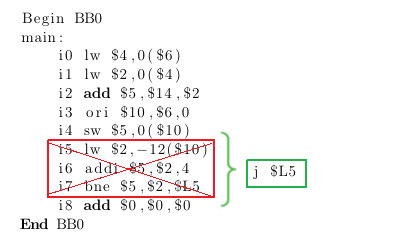
\includegraphics[scale=0.8]{images/BB0TD2.png}~\\[1.5cm]
    
    En répliquant le test "\textbf{test\_all\_together.cpp}" on arrive à avoir un gain de 2 cycles avec le scheduling. Cependant on ne retrouve aucune différence en appliquant le Renommage \& le scheduling en même temps, de même si on applique seulement le Renommage.
    
    \item La deuxième remarque concernant la liste des registres disponibles pour le renommage. Avant chaque renommage on construit une liste de registres utilisables pour le renommage des registres. En comparant les blocs de base pour les fichiers plus volumineux (\textit{aes\_O0.s}) on a remarqué que le peu de registre disponible nous pose problème. Ainsi l'optimisation à apporter consisterait à trouver un meilleur algorithme qui permet de calculer plus de registres utilisables.
\end{enumerate}

\section{Synthèse}
 
On teste et on vérifie manuellement les fichiers suivants (test\_td2.s | ex\_simple.s et dep\_inst.s) .

On peut en tirer les conclusions suivantes

\begin{itemize}
    \item Le renommage ne fait jamais perdre de cycle.
    \item Le renommage de registre est inutile sans ré-ordonnancement (0 cycle gagné).
    \item Les gains du ré-ordonnancement sont aussi faible que le renommage de registres avec les petits fichiers.
\end{itemize}

Les points les plus importants que nous retenons pour l'optimisation du nombre de cycles sont:
\begin{itemize}
    \item L'étude plus approfondie des instructions entre elles, ainsi les éliminer dans le cas où elles n'ont pas d'impact dans le code ou  qui sont répétitives (comme vu dans l'exemple ci-dessus).
    \item L'amélioration de la construction de la liste des registres utilisables pour le renommage.
\end{itemize}

\section{Conclusion}


Nous avons implémenté avec succès toutes les fonctions de traitement du code ce qui nous a permis de discuter des éventuelles optimisations qui permettrait un gain du nombre de cycles, malheureusement nous n'avons pas pu les implémenter.

Grâce à ce projet, nous avons approfondi notre compréhension des opérations se passant à bas niveau ce qui nous a permis de mieux comprendre le fonctionnement et les enjeux de la compilation.

\newpage
\appendix
\section{Annexe}
\subsection{test\_td.s (code assembleur vue en td2)}
\label{chap:TestTd2}

\begin{lstlisting}
	.text
	.ent main
main:	
	lw $4, 0($6)
	lw $2, 0($4)
	add $5,	$14, $2
	ori $10, $6, 0
	sw $5, 0($10)
	lw $2, -12($10)
	addi $5, $2, 4
	bne $5, $2, $L5
	add $0, $0, $0

$L4:
	lw $4, 0($6)
	lw $2, 0($7)
	add $5, $4, $2
	sw $5, 0($6)
	addiu $12, $8, 2
	addiu $7, $12, 1
	bne $7, $0, $L5
	add $0, $0, $0
	
	sub $6, $0, $5
	sll $6, $3, 4
	addiu $5, $6, -2
	sw $15, 12($7)
	sw $10, -4($6)
	j $L4
	add $0, $0, $0
	
$L5:	
	sub $8, $10, $15 	
	sll $10, $10, 4	
	sw $8, 8($7)	
	add $10, $8, $10	
	sw $10, 12($7)
	jr $31
	add $0, $0, $0

	.end main
	.set reorder
\end{lstlisting}


\subsection{CFG}
\label{chap:cfg}

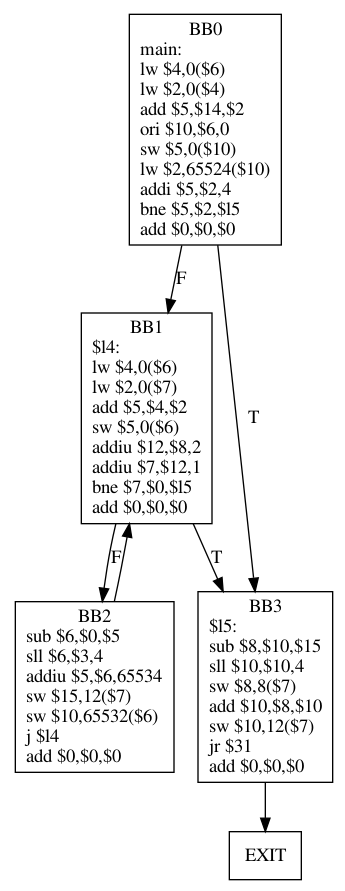
\includegraphics[scale=0.6]{images/cfgTD2.png}~\\[1.5cm]

\subsection{Dependance instructions BBO TD2}
\label{chap:Dep}

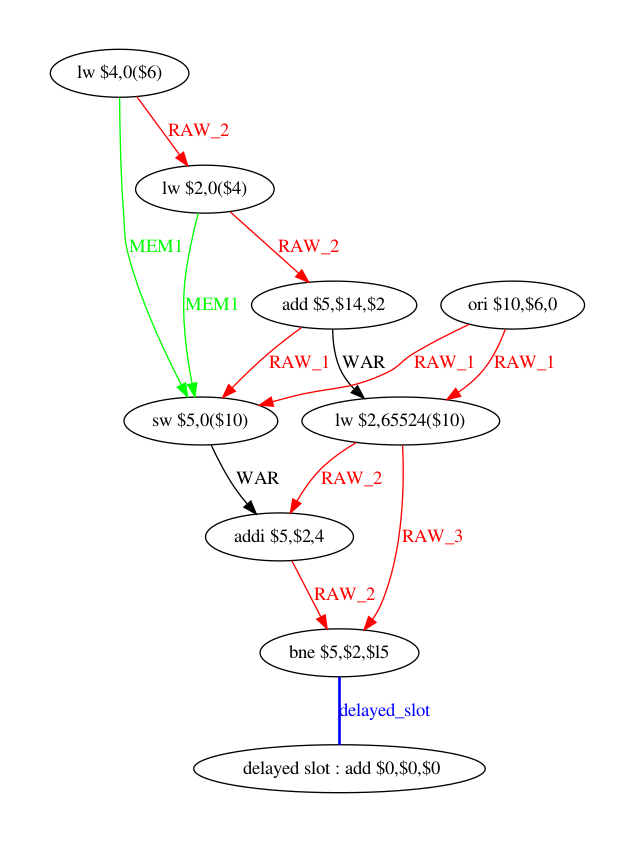
\includegraphics[scale=0.6]{images/depBBOtd2.png}~\\[1.5cm]

\end{document}
